\documentclass[twoside,twocolumn]{article}

\usepackage{blindtext} 
\usepackage{graphicx}
\usepackage[sc]{mathpazo} 
\usepackage[T1]{fontenc} 
\linespread{1.05} 
\usepackage{microtype} 


\usepackage[english]{babel} 


\usepackage[hmarginratio=1:1,top=32mm,columnsep=20pt]{geometry} 
\usepackage[hang, small,labelfont=bf,up,textfont=it,up]{caption} 
\usepackage{booktabs} 


\usepackage{lettrine} 


\usepackage{enumitem} 
\setlist[itemize]{noitemsep} 


\usepackage{abstract} 
\renewcommand{\abstractnamefont}{\normalfont\bfseries} 
\renewcommand{\abstracttextfont}{\normalfont\small\itshape} 


\usepackage{titlesec} 
\renewcommand\thesection{\Roman{section}} % 
\renewcommand\thesubsection{\roman{subsection}} 
\titleformat{\section}[block]{\large\scshape\centering}{\thesection.}{1em}{} 
\titleformat{\subsection}[block]{\large}{\thesubsection.}{1em}{} 


\usepackage{fancyhdr} 
\pagestyle{fancy} 
\fancyhead{} 
\fancyfoot{} 
\fancyhead[C]{ Unidad I : Articulo del Proyecto ICCAPJ $\bullet$ Septiembre 2020 $\bullet$ } 
\fancyfoot[RO,LE]{\thepage} 


\usepackage{titling} 


\usepackage{hyperref} 


%----------------------------------------------------------------------------------------
%	TILULOS
%----------------------------------------------------------------------------------------


\setlength{\droptitle}{-4\baselineskip} 

\pretitle{\begin{center}\Huge\bfseries} 
\posttitle{\end{center}} 
\title{Implementación de Call Center y asistencia para el poder judicial} 
\author{Samuel Nuñez Mamani - Franklin Carlos, Huichi Contreras, \\
Anthony Robles Flores. }
\date{\today} 
\renewcommand{\maketitlehookd}{
\begin{abstract}
\noindent 
Determino las estrategias que debiera tenerse en cuenta para planificar, estructurar y finalmente escribir un articulo o “paper” de Ciencias Sociales
conforme a la Asociacion Americana de Psicologa (APA) Sexta Edicion. Se pretende que el lector produzca su propio trabajo.
\end{abstract}
\begin{abstract}
\noindent 

Treva es un sistema enfocado en los formularios de satisfacion del cliente en donde el propietario podra generar formularios y enviar cada cierto tiempo a sus empleado o interesados para que puedan llenarlo segun
las opciones que cuenta el formulario, a partir de esos datos podemos al propietario dar estadisticas en la cual puede verificar que opciones escogieron los clientes o empleados, y aparte de ello podemos analizar los datos
para dar recomendaciones o proyecciones estimadas de areas especificas.

\end{abstract}
}

%----------------------------------------------------------------------------------------

\begin{document}

% Print the title
\maketitle

%----------------------------------------------------------------------------------------
%	INTRODUCCION
%----------------------------------------------------------------------------------------

\section{Introduccion}
\lettrine[nindent=0em,lines=3]{A}ctualmente en el Perú las pequeñas y medianas empresas producen al mercado peruano ingresos y empleo, la gran cantidad de informacion que manejan es debido al alto numero de operaciones que realizan a diario, por lo tanto se necesita una forma de controlar los datos como las opiniones de los clientes y de esta forma conseguir retroalimentacion instantanea para las empresas. Asimismo tener la informacion en reportes descriptivos para la visualizacion se ha hecho parte importante de los sistemas de hoy para tomar desiciones acertadas y utiles para las empresasl.

\section{Titulo}
El sistema se identifica con el titulo de treva.

\section{Autores}
\begin{itemize}
\item Anthony Richard , Robles Flores.
\item Franklin Carlos, Huichi Contreras.
\item Samuel, Nuñez Mamani.
\end{itemize}

\section{Planteamiento del problema}
\subsection{Problema}
La problematica general es el como las empresas evaluan el desempeño de sus servicios, y como pueden medir la satisfacción del cliente al igual de saber la efectividad y el buen manejo de sus productos.

\subsection{Justificacion}
Hoy en día los datos toman cada vez mas valor en una organizacion o empresa, de esta manera pueden asegurar una ventaja contra sus competidores y así beneficiarce para obtener una mejor calidad de servicio, mejorar su producto y por consiguiente clientes satisfechos.

\subsection{Alcance}
Para el alcance de este proyecto nesecitaremos de clientes que quieran realizar sus formularios de satisfaccion y ofrecerles todas las herramientas nesecarias para que lo hagan de manera eficaz. Alcanzado la meta podremos generar los dashboards que ayude al cliente a ver los resultados entre otros indicadores.


\section{Objetivos}
\subsection{General}
Determinar el nivel de satisfaccion de los clientes de las empresas afiliadas a treva

\subsection{Especificos}
\begin{itemize}
\item Mejorar el rendimiento de las empresas con reportes estadisticos en las encuestas realizadas sobre el nivel de satisfaccion de los clientes, que se usaran para la toma de desiciones.
\item Comparar los grados de satisfacción de los clientes periodicamente.
\item Definir la relación real entre encuestas y satisfacción del cliente.
\end{itemize}

\section{Referentes teoricos}
La idea nos nacio como grupo luego de ver ejemplos de paginas como bimatico en donde manejaban estadisticas de la realizacion de las estadisticas de cada pregunta y area realizada
a continuacion pondre un ejemplos realizados esta pagina. Apartir de esas estadisticas nos dimos cuenta que pdoriamos realizar un sistema que pueda controlar todo esto desde el punto inicial hasta llegar al punto de los reportes.
\begin{figure}[h!]
	\begin{center}
		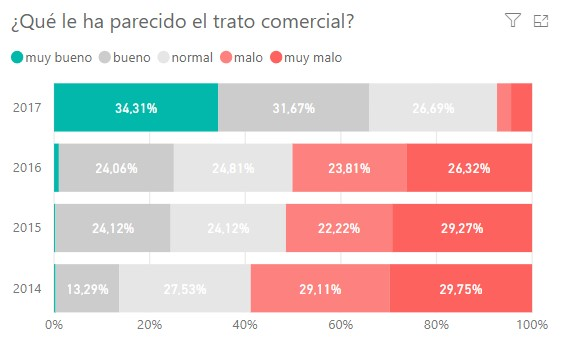
\includegraphics[width=7.5cm]{./Imagenes/esta1} 
		\caption{Estadistica de bimatico}
	\end{center}
\end{figure}
\begin{figure}[h!]
	\begin{center}
		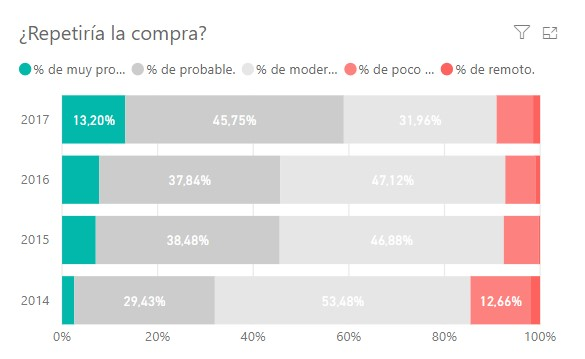
\includegraphics[width=7.5cm]{./Imagenes/esta2} 
		\caption{Estadistica de bimatico}
	\end{center}
\end{figure}
\begin{figure}[h!]
	\begin{center}
		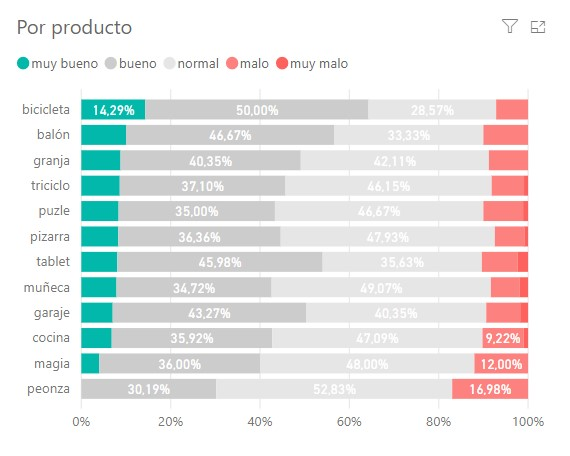
\includegraphics[width=7.5cm]{./Imagenes/esta3} 
		\caption{Estadistica de bimatico}
	\end{center}
\end{figure}

\section{Desarrollo de la propuesta}
Para solucionar esta problematica existente en el poder judicial tomando en cuenta estos tiempos de la pandemia donde el asilamiento social a provocado un desvalance en las actividades normales de los trabajadores en esta entidad sobrecargando con labores adicionales para el proceso de adaptamiento a este contexto en el que vivimos , la implementacion de un Call Center podria agilizar los procesos de los trabajadores donde un asistente podria solucionar las interrogantes que podrian tener los usuarios antes que un trabajador interno pueda intervenir, pero en caso el asistente no pudiese resolver esta duda , el mismo call center podria derivar a un anexo a poder comunicarse via telefonica con un asesor legal.
\\
Viendo que existen diferentes canales de comunicacion,  en el momento de interactuar con el usuario , proponemos tambien una aplicacion Movil en Android donde este prodra otorgar los mismos servicios añadiendo tambien la facilidad al usuario de poder ubicar las oficinas de acuerdo a la sucursal en la que necesiter asistir a una cita programada , como tambie  el llenado de formularios con formatos ya establecidos por el poder judicial donde hay algunos documetos que no se necesiten la evaluacion de un abogado y como resultado la aplicacion podria descargar un PDF con los datos solicitados usando el formato de documentos del Poder Judicial.
\\
Tomando en cuenta que la tecnologia de tener un SmartPhone invade cada vez mas a la sociedad , incluir un módulo en el aplicativo acerca de las audiencias que el poder judicial publicará asi el usuario externo podría tener a la mano esta información a fin de poder asistir y estar pendientes puesto que en la web se encuentra el cronograma pero ubicar una audiencia para aquellos que desconocen el uso de una plataforma web podria ser dificultoso , la aplicacion movil podria ayudar a que sera mas sencillo y rápido de identificar una audiencia.

\subsection{Tecnologia de informacion}
En esta seccion definiremos las herramientas que se utilizaran para el desarrollo del proyecto asi mismos las plataformas que se emplearan para las conexiones en algunos servicios.
\begin{itemize}
\item Plataforma Colaborativa
\subitem Github
\subitem Google Meet
\subitem Teams Microsoft
\item Base de Datos:
\subitem Firebase.
\item Lenguajes de programación:
\subitem Java.
\item Asistente Virtual:
\subitem DialogFlow.
\item Red Telefonica:
\subitem VoximPlant.
\end{itemize}

\subsection{Metodología}
La metodologia que usaremos será RUP (Proceso Unificado de Rational)puesto que esta metodología provee un entorno de desarrollo flexible basado en estándares que se adapta a las necesidades del desarrollador o de las empresas y tener la facilidad de dividir todas las actividades de forma de que a cada participantele pueda tocar la parte que le compete.



\section{Desarrollo de Solución de Mejora}

\subsection{Casos de Uso de la aplicación}
\begin{figure}[h!]
	\begin{center}
		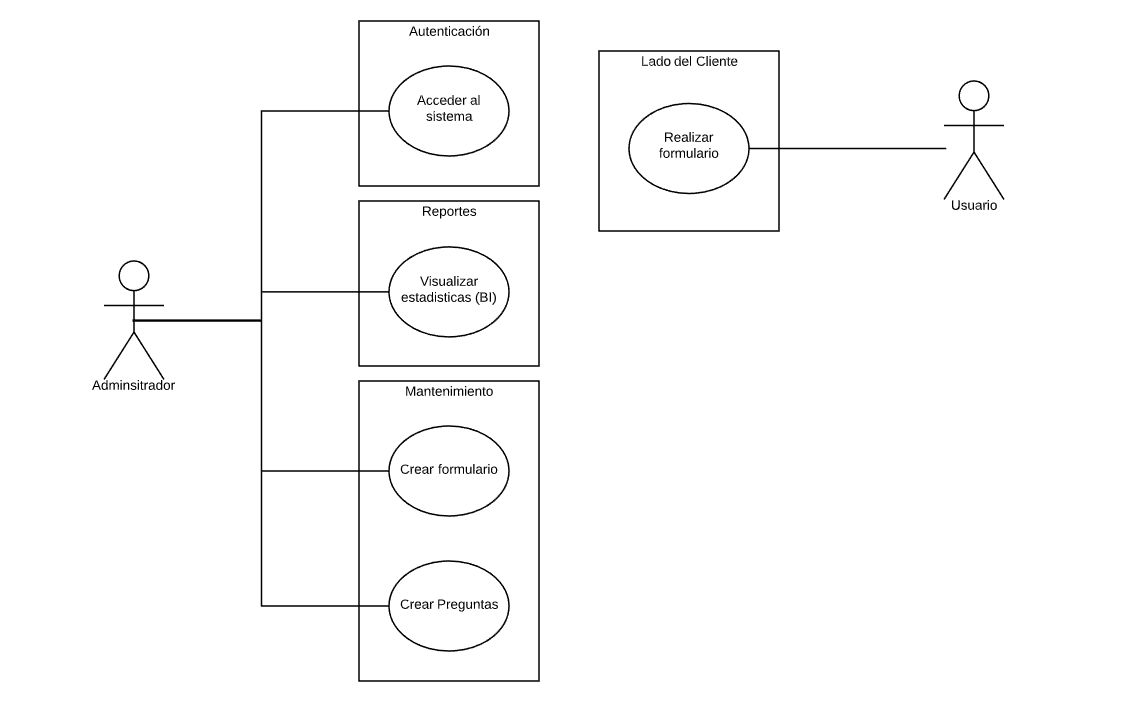
\includegraphics[width=7.5cm]{./Imagenes/use_case} 
		\caption{Use case}
	\end{center}
\end{figure}

\subsection{Diagrama de Arquitectura de la aplicación}
Diagrama de Arquitectura de la aplicación
\begin{figure}[h!]
	\begin{center}
		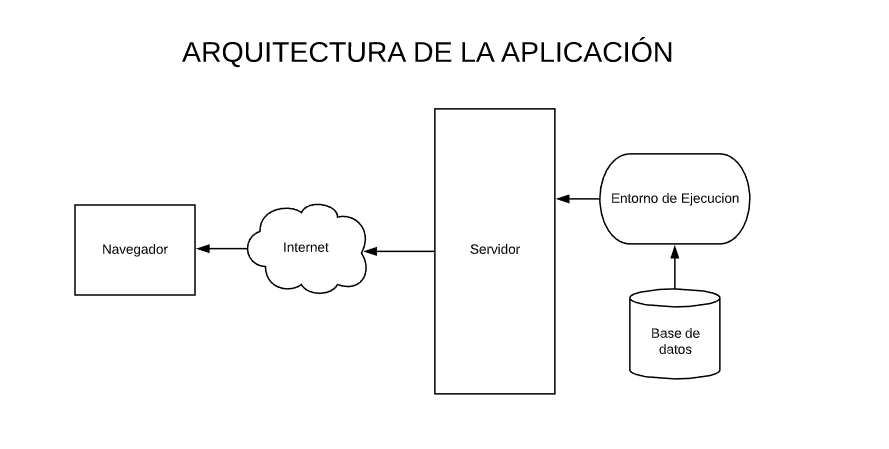
\includegraphics[width=7.5cm]{./Imagenes/bd_architecture} 
		\caption{bd architecture}
	\end{center}
\end{figure}

\subsection{Diagrama de Clases de la aplicación}
Diagrama de Clases de la aplicación
\begin{figure}[h!]
	\begin{center}
		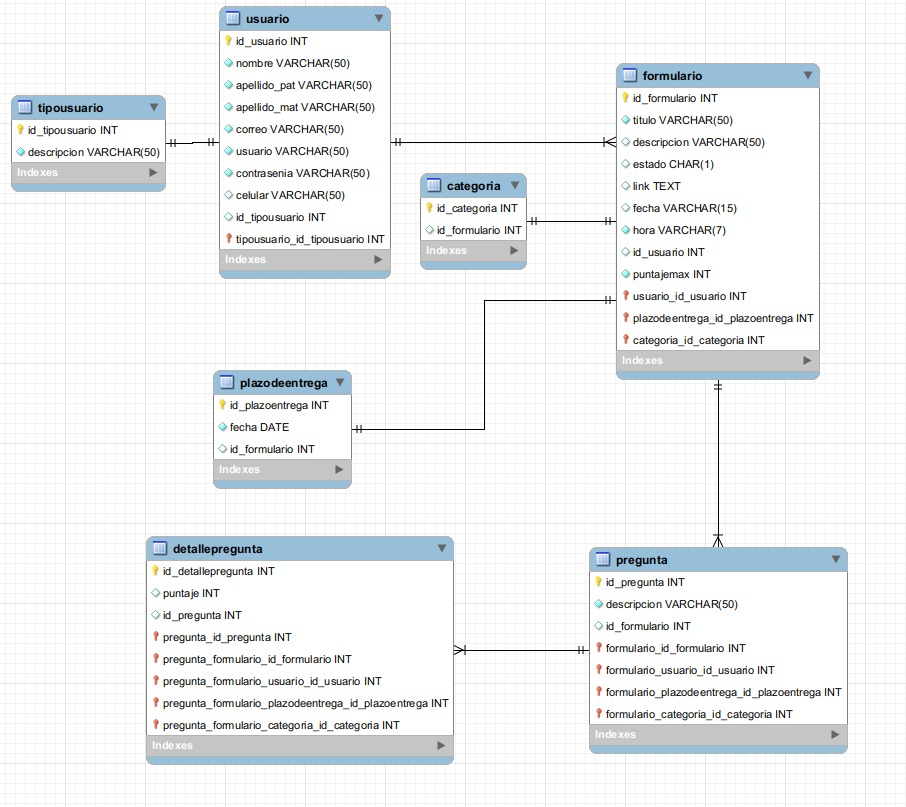
\includegraphics[width=7.5cm]{./Imagenes/diagramclass} 
		\caption{Diagram Class}
	\end{center}
\end{figure}



\end{document}
